
\section{Chapter Overview}

This chapter will focus on the design of the system. Using the different types of UML diagrams and Graphical User Interface (GUI) images, we aim to illustrate certain sections of the software explaining in detail how they were designed. This section outlines this in different categories. 
\section{Model-View-Controller}
The Software design pattern that we chose was a Model-View-Controller(MVC). We felt it was best for the task ahead as the two of us had past experience using MVC design patter to develop work. We also believed that it would be perfect to connect the various parts of the project together while also keeping an internal separation for the representation of all of the different modules, finally we felt that since MVC is a pattern that is usually used in the designing layouts of the pages this would be essential in the presentation of the project.

\section{Component Diagram}

The component diagram in figure 5.1 shows the structural relationship between the components in the system. The diagram illustrates the usability of the different components of derivatives of system requirements while installing the software.
\begin{figure}[h!]
	\caption{Component diagram.}
	\label{image:myImageName}
	\centering
	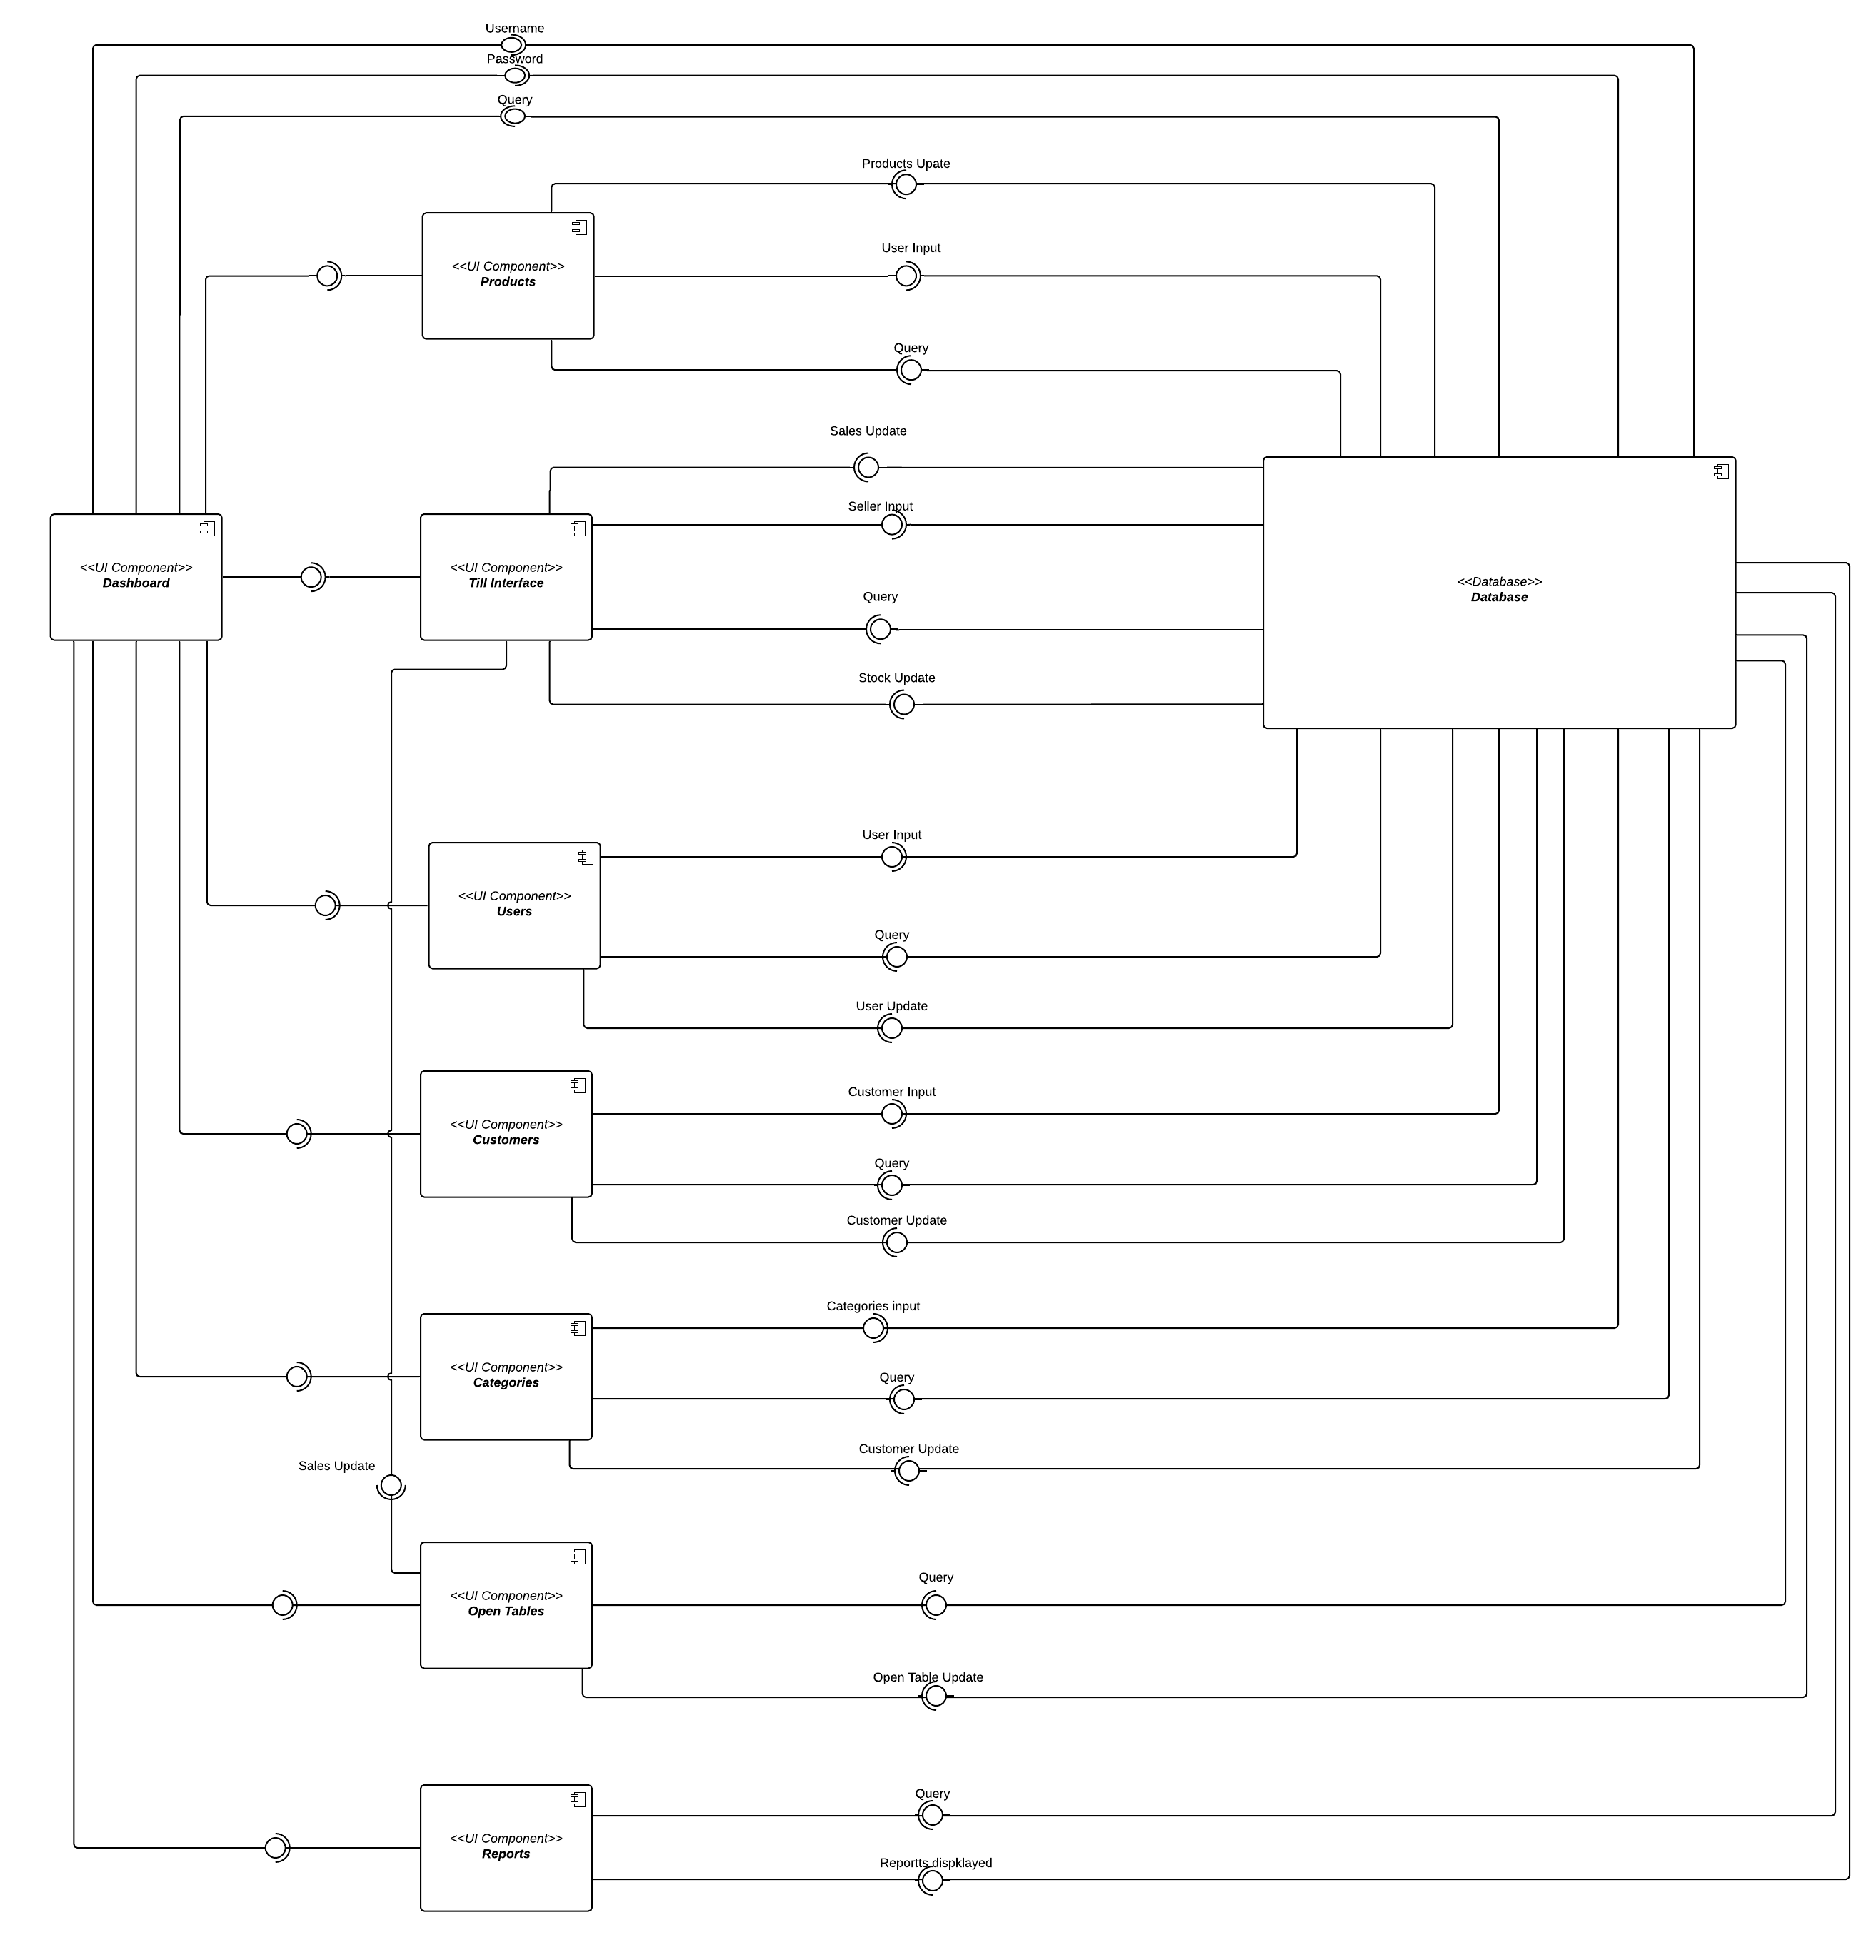
\includegraphics[width=0.9\textwidth]{Fig images/POS Component.png}
\end{figure}
\section{Data Storage}

Data storage is a key part of this project. While choosing our database, we reviewed several storage solutions. This is a must-have in any system since we are dealing with offline complex data. The database choice is therefore critical for the preservation of data \cite{DS}. The following is a brief synopsis of the storage solution we chose and why we decided to pick it:
Relational Database Management System (RDBMS) 

\section{Relational Database Management System (RDBMS)}

A Relational Database Management System (RDBMS) is a database management system based on the relational model of data. This particular type of database enables a user to access data based on its relation to another piece of data \cite{CODE}. This ensures that is secure and a clear record of modification, read or write is maintained. It is fast and reliable and often used by some of the biggest companies in the world. It provides the developer with an option to use a structured query language (SQL) for querying and maintaining the database. 
\newline
\newline
This is especially important since MySQL is an open-source programming language. The language is widely used by different developers and has been operation since 1995 \cite{CODE}. This means that the code is widely re-usable and can get updates from different developers. It also assists the developers to raise a quorum on an impending challenge where they can get assistance from far wide in the information technology industry. 
\newline
\newline
RDBMS’s are often open-source and free to use. You can, however, opt to use paid solutions such as Oracle and SQL Server. The paid solutions versions are more utilitarian with options such as tech support.  Oracle, for instance, is not an open-source software \cite{ORA}. The database is expensive as well and is used often for huge amounts of data with very poor scalability. This, therefore, disqualifies these types of the database since they don’t provide the necessary utilities for our project. Ideally, the paid solutions are unrestricted versions of the default open-source version. 
\newline
\newline
RDBMS has several constraints that are beneficial to our project. This is; Not Null. This constraint ensures that there are no null/empty values in the columns. Unique. As the name suggests, the unique constraint is used to ensure all the data in the columns is unique. Check. The constraint is built to ensure that all the data in the individual columns meet a particular predefined condition. Primary key.  The primary key must be unique. This constraint must be unique since it is used to uniquely identify the different rows in a table. The key is also used to link a table to another. It, therefore, cannot have a null value. Foreign Key. This constraint is used to link two tables where one must behave the Primary key. Data Integrity. This constraint is used to ensure there is data integrity before modifying, writing, reading, or creating data \cite{RDBMS}. There are several categories that a single task must pass to ascertain data integrity. The categories are; Entity Integrity, Referential Integrity, Domain Integrity, and User-Defined Integrity. \cite{RDBMS}
The above constraint contributed effectively to the advantages of the database.  As a result, the RDMS database enshrines the following advantages:

\subsection{Data Structure}

As defined above, tables and columns are a defining factor in the database. This is an important figure since it provides the user with a natural space where data is structured and organized \cite{ADB}. This makes it easy to structure queries to such through columns for matching entities. 

\subsection{Privileges}

This feature is imported into our system. It assists the developer in categorizing access to sensitive information. The feature allows the database administrator to control activities in the database. This is achieved through integrity frameworks such as atomicity, consistency, isolation, and durability \cite{WRD}.

\subsection{Data Recovery}

Data loss is not a unique narrative in any information technology field. Data loss is, therefore, an impeding risk while implementing any technological platform associated with data. RDMS leverage on this risk by providing the users with period backups of the system. This is preset by the developer to ensure the database periodically keeps a backup. 

\subsection{Flexibility}

The database has been developed to accommodate different types of applications. This means that different applications based on different platforms can be used to access the platform. It further makes it easier for developers to handle big data. 

\subsection{Data Consistency}
RDBMS databases are developed with a normalization feature. This ensures that all the tables maintain a proper structure of rows and columns. This also helps in sorting data where there predetermined methodologies of sorting data. 

\subsection{Speed}

RDMS cannot be argued as the fastest database. The platform, however, provides several trades off that make it the best utilitarian for speed. RDMS provides a cheap data storage option. This means that by combining a large version of the same, the processor speed, decreasing memory requirements, and scaling makes RDBMS the most convenient database for the project. This is based on the tradeoff of the project as a whole \cite{ADB}.

\subsection{Ease of Use}
The platform supports MySQL. This is a very simple syntax language that eases the development work. The syntax used standard English language keywords and phrasing hence being very easy to use, learn, and intuitive. 

\section{Why RDBMS}

SQL is an extremely flexible and robust querying language. When researching for a suitable query-based database, we come across RDBMS that provided all the utilities that we required. This was the best platform considering our application was largely a data computation and storage unit. WE, therefore, required a database that was easily designed while capable of handling complex systems. We, therefore, decided RDBMS is the best fit for our needs
\newline
\newline
The next step was to decide on the type of RDBMS to use. As mentioned above there are many open source RDBMSs available for developers.  While there we rational versions of the same, we have used MySQL before and were aware of its capabilities. We, therefore, picked the same to manage the learning curve in the entire project.
\newline
\newline
While this was the case, there several pointers that ruled out RDBMS as the best database option. This as listed by an online editorial include; 

\begin{itemize}
    \item Data Safety
    \item Fault-Tolerant 
    \item Ease of use
    \item Scalability 
\end{itemize}


\section{Entity Relationship Diagram} 

An Entity Relationship Diagram (ERD) shows the relationships of components stored in a database and is often used to represent a relational database and its requirements in a top-down view. We developed this diagram as a reference point considering the complexity of our project. Besides this, the diagram was developed as an industrial standard ensuring the code was readable to future users or introduced developers. The following ERD, figure 5.2, is the database schema for our POS system.

\begin{figure}[h!]
	\caption{Database schema.}
	\label{image:myImageName}
	\centering
	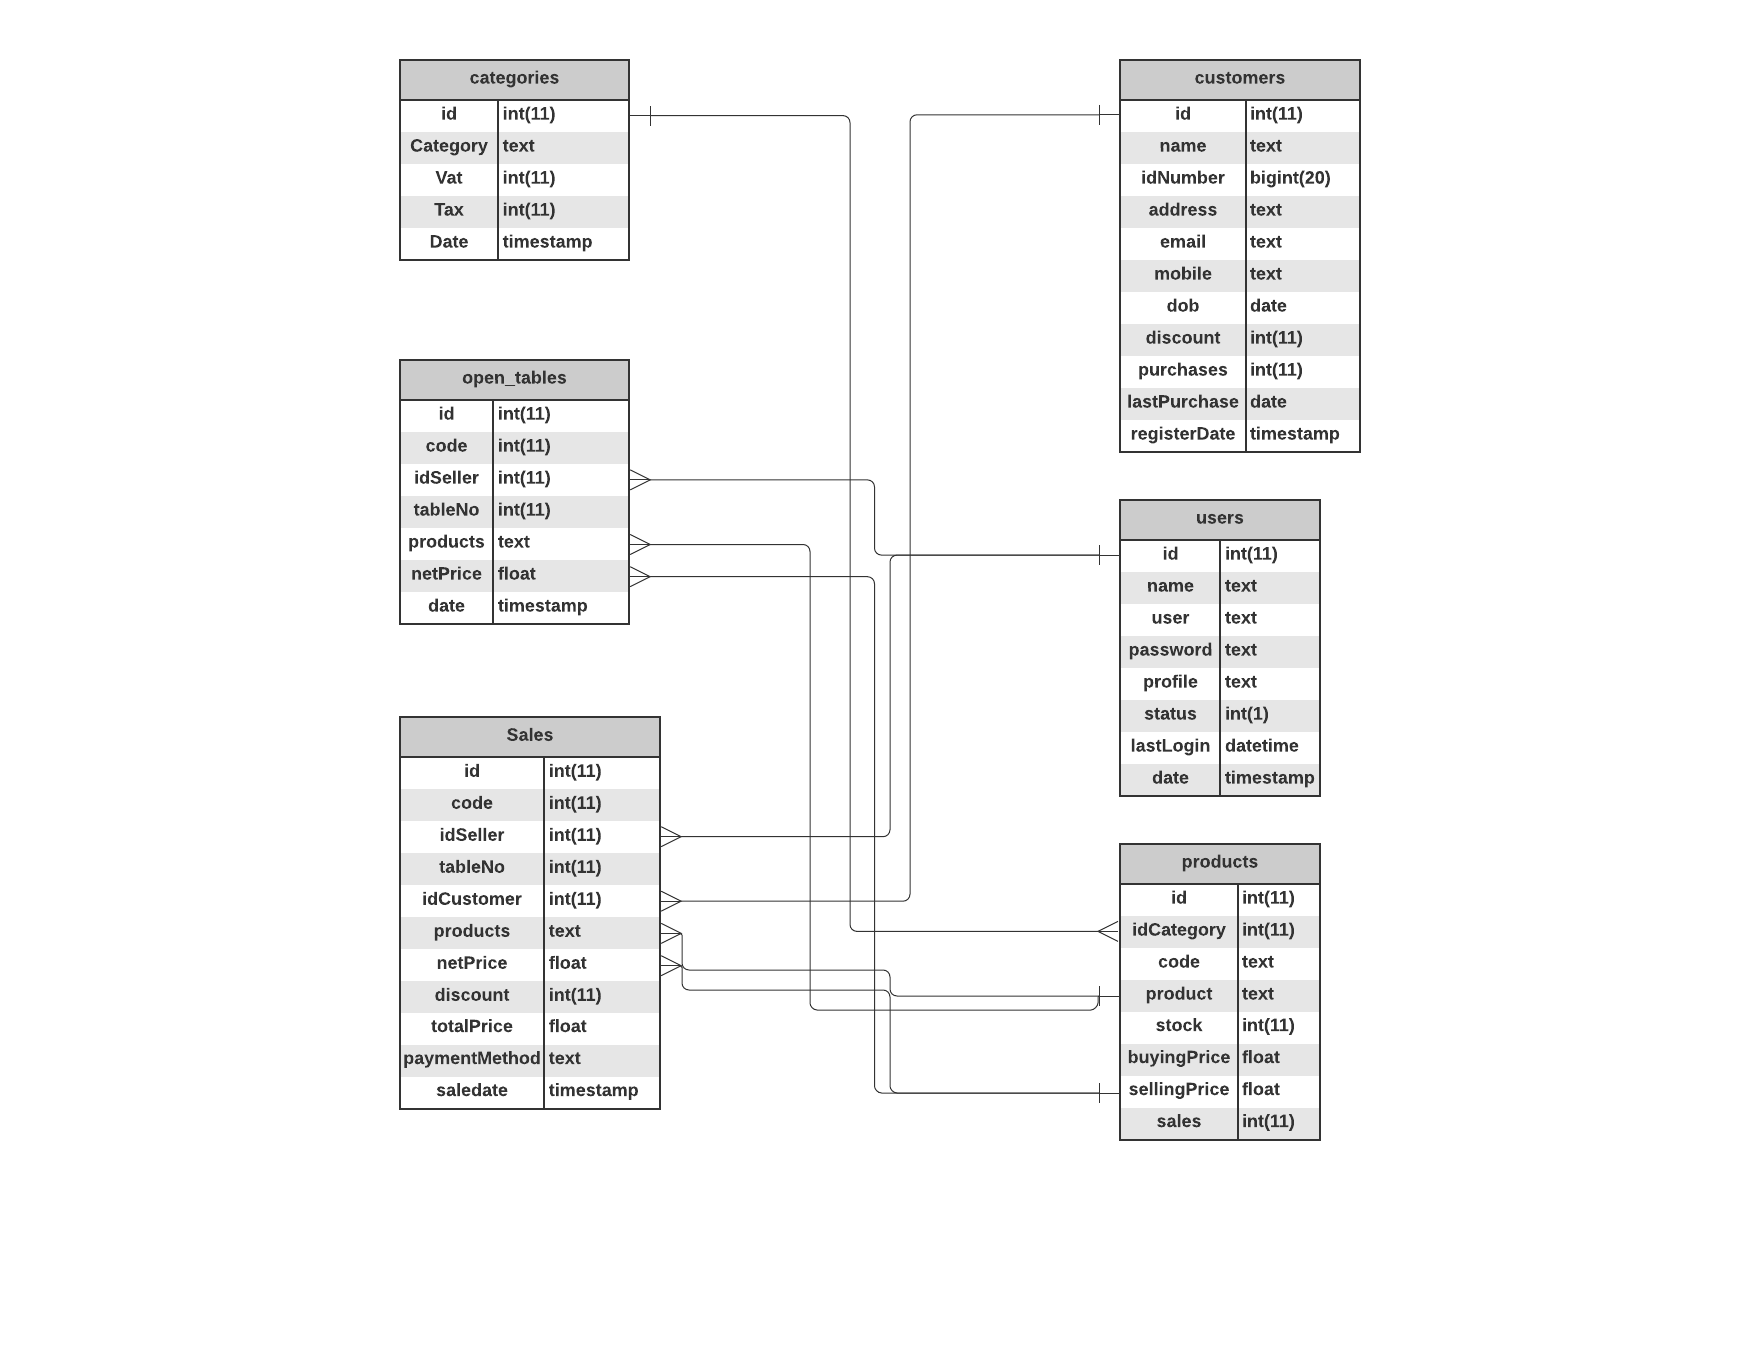
\includegraphics[width=0.9\textwidth]{Fig images/database schema.png}
\end{figure}

\section{Database Design}

At the start of the project, before a single line of code was written, a plan was put together for the database. The database is a key element to the system so the structure had to be designed well in advance of any coding. We had to make sure that the database captured all necessary information and was interconnected sufficiently to allow efficient querying. We also had to make sure the database was secure considering the environment that the software was to be placed in. Since the system was developed to manage the business as well as payments, the database design concepts were reviewed in different scenarios 

Concepts of the database design are as follows;

\begin{itemize}
    \item Ability to store product details.
    \item Ability to control the stock of the products when putting into an order.
    \item Ability to alter stock levels with new stock purchases.
    \item Ability to add and control customer details.
    \item Ability to add and control staff details.
    \item Ability to add and control category details.
    \item Ability to add and control the sale and open sale details.
\end{itemize}


\section{Graphical User Interface}

A major part of our system aims was to make it as efficient and as user friendly as possible. The graphical user interface (GUI) is the only component of the system that the user interacts with and therefore it is of great importance. The design had to be simple, clear, and concise but also have all of the required features needed at the users' fingertips. This is an important feature since it elevates the practicability of having features from two different platforms merged into one. We, therefore, had to make sure the two different components don’t up complicate the system.
\newline
\newline
One of the main objectives of this project was to create a system that allowed users to complete orders in a fast and efficient manner. This was judged by the number of clicks required to get from the start of an order to the finish as well as the time taken to do so. Using AdminLTE, with a little tweaking offered us the ability to achieve our goals. The platform also enabled us to save time that would be spent developing the extensive user interface. Within our system, there are two different GUIs with each requiring a different design specification.

\subsection{Till GUI}

The system GUI is a critical part of this project. The usability and ease of usage, therefore, remained a part of the highest priority. The GUI is one of the main characteristics of the system. Through this portal clients would be required to make payments or orders for different assortments. The till portal was, therefore, design with the users' perspective in mind. We developed this section of GUI to be simplistic and intuitive. This means that a new user would have the easiest time figuring out how the portal works. We further made sure that the GUI did not require a lot of hardware resources which would end up slowing the entire system. We, therefore, developed several guidelines that would ensure we developed the correct till GUI.
\newline
\newline
The following is the specification for the till GUI: 
\newline
\newline
Minimum clicks from start to finish.  This would ensure that a new client would be able to easily navigate through the system without assistance. It would further ensure that a company is capable of maintaining its clients.  
Every option is as little clicks away as possible. This would reduce the stress of constantly asking for help. It would also reduce the chance of clients finding the application cumbersome. 
\newline
\newline
Adding products confined to half of the GUI while the payments process is confined to the other half. This ensures that the clients will have an easy time understanding the logic of the application. It further means that the clients will be able to navigate through the application by accessing portals that they require for transactions.
\newline
\newline
Accessing sales and open tables is in the sidebar of the GUI. This as well ensured that the clients did not have to scroll through different options to make an order. It further ensured that adding orders or modifying one was easy and convenient. 
\newline
\newline
Ability to fit on any monitor size. Since practicability is one of our main objectives, we made sure that the system is scalable and compatible with different devices and operating systems. This enables clients with different preferential payments method to make payments from their different devices with ease. It also enables the developers to explore different platforms that the system can be upgraded to.
\newline
\newline
One-click payment method. This is one of the main objectives of the system. One-click payments reduce the amount of time and complexity of the system. Providing the user with complex computational power with the most friendly GUI. This improves on the operations at the different facilities while improving sales and management utilities. 
\begin{figure}[h!]
	\caption{Till GUI}
	\label{image:myImageName}
	\centering
	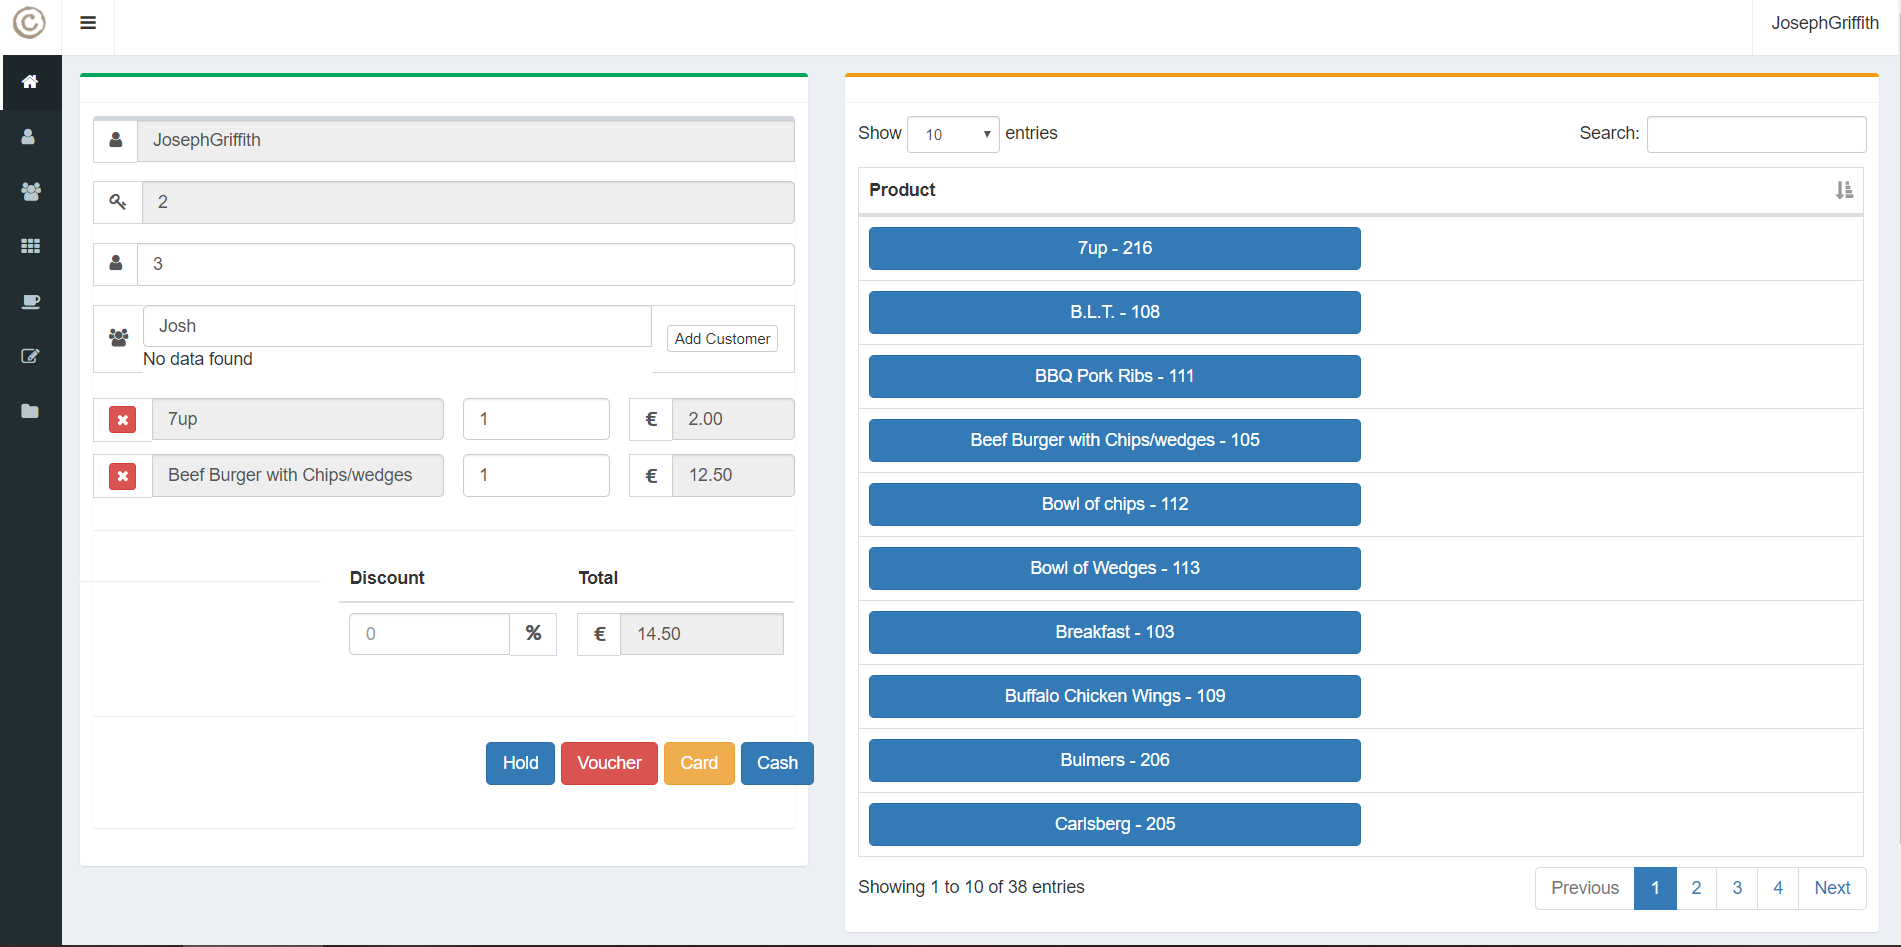
\includegraphics[width=0.9\textwidth]{Fig images/tillGUI.PNG}
\end{figure}

show a design of the order the GUI uses to abide by the specifications listed above. Each part of the process is kept to one side of the till. Adding products on sale is situated on the right-hand side whereas the product list, table number, customer data, discount, and payment methods are all conducted on the left.
\newline
\newline
The sidebar allows the user to access sales and open tables to process table sales. Because of the need for use on tablets the system is designed to allow the GUI to fit all size screens. This allows the easy use of remote ordering.

\subsection{Management GUI}

The management system requires a GUI to input data into various fields and therefore requires an appropriate input design. Using AdminLTE as our template we were able to re-use the same layout for each of the required fields (users, categories, products, and customers). The use of this platform enabled as to focus on the back-end ingenuity to provide the users with the best experience. Further, the platform enabled us to develop a complex GUI that is differentiated from the till GUI. The management GUI further was required to provide a detailed overview of the operations in the restaurant. This portal, therefore, required careful handling ensuring critical elements of the restaurant were easily accessible. Further, the management would have an easy time viewing the different entity values. 
\newline
\newline

\begin{figure}[h!]
	\caption{Side tabs.}
	\label{image:myImageName}
	\centering
	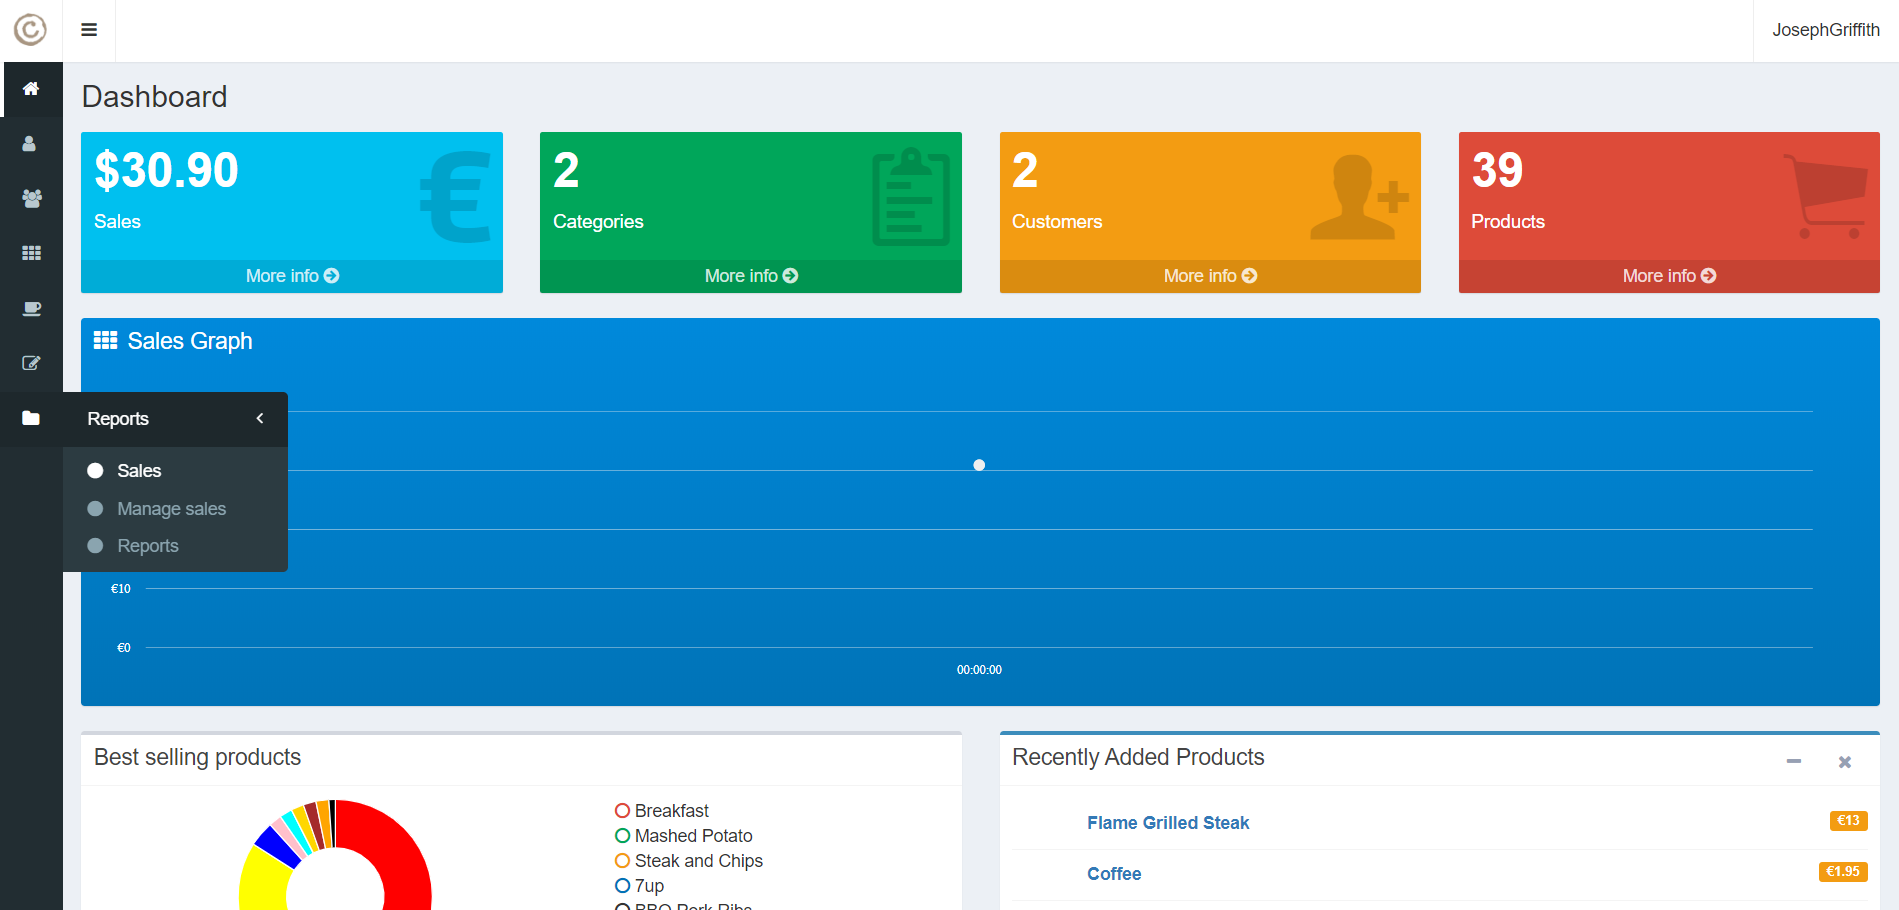
\includegraphics[width=0.9\textwidth]{Fig images/sidetab.png}
\end{figure}
  Figure 5.4 shows the design of the management application with the different functions appearing down the left-hand side as a tab. Each tab contains a sub-form with Figure 6.1/6.2 containing the structure of the generic data input form.
  
\section{Pricing}

There are many factors throughout the system that affect the pricing of an item. The following is a list of the modules that affect pricing and how they all come together to make the price of a product:
First of all, starting with categories, when adding a category, the owner/manager is asked to enter the percentage VAT and Tax rate of this particular category.
\newline
\newline
Secondly when adding a product the user chooses the product category and inserts the cost price. The VAT and Tax are automatically added to this price and are displayed to the user.
The user then has the option of adding a percentage mark-up, chosen by themselves to the price or, they can choose to put their selling price into the system. 
\newline
\newline
This process offers the user a lot of flexibility as well as efficiency. By just entering the cost price of a product the system computes this automatically. This process can save the user a lot of time spent calculating rates and mark-ups while reducing the risk of errors on their part. This further enables the management to work on different discounts and offers. By integrating the same in the system, this allows the user to feel more comfortable while making an order and to plan future visits to the restaurant. Using the system also enables the management to react to the demand in the market more easily. 

\section{Flow Charts}

The following diagram is a flow chart of how the entire system works.
\begin{figure}[h!]
	\caption{Flow chart of the entire system.}
	\label{image:myImageName}
	\centering
	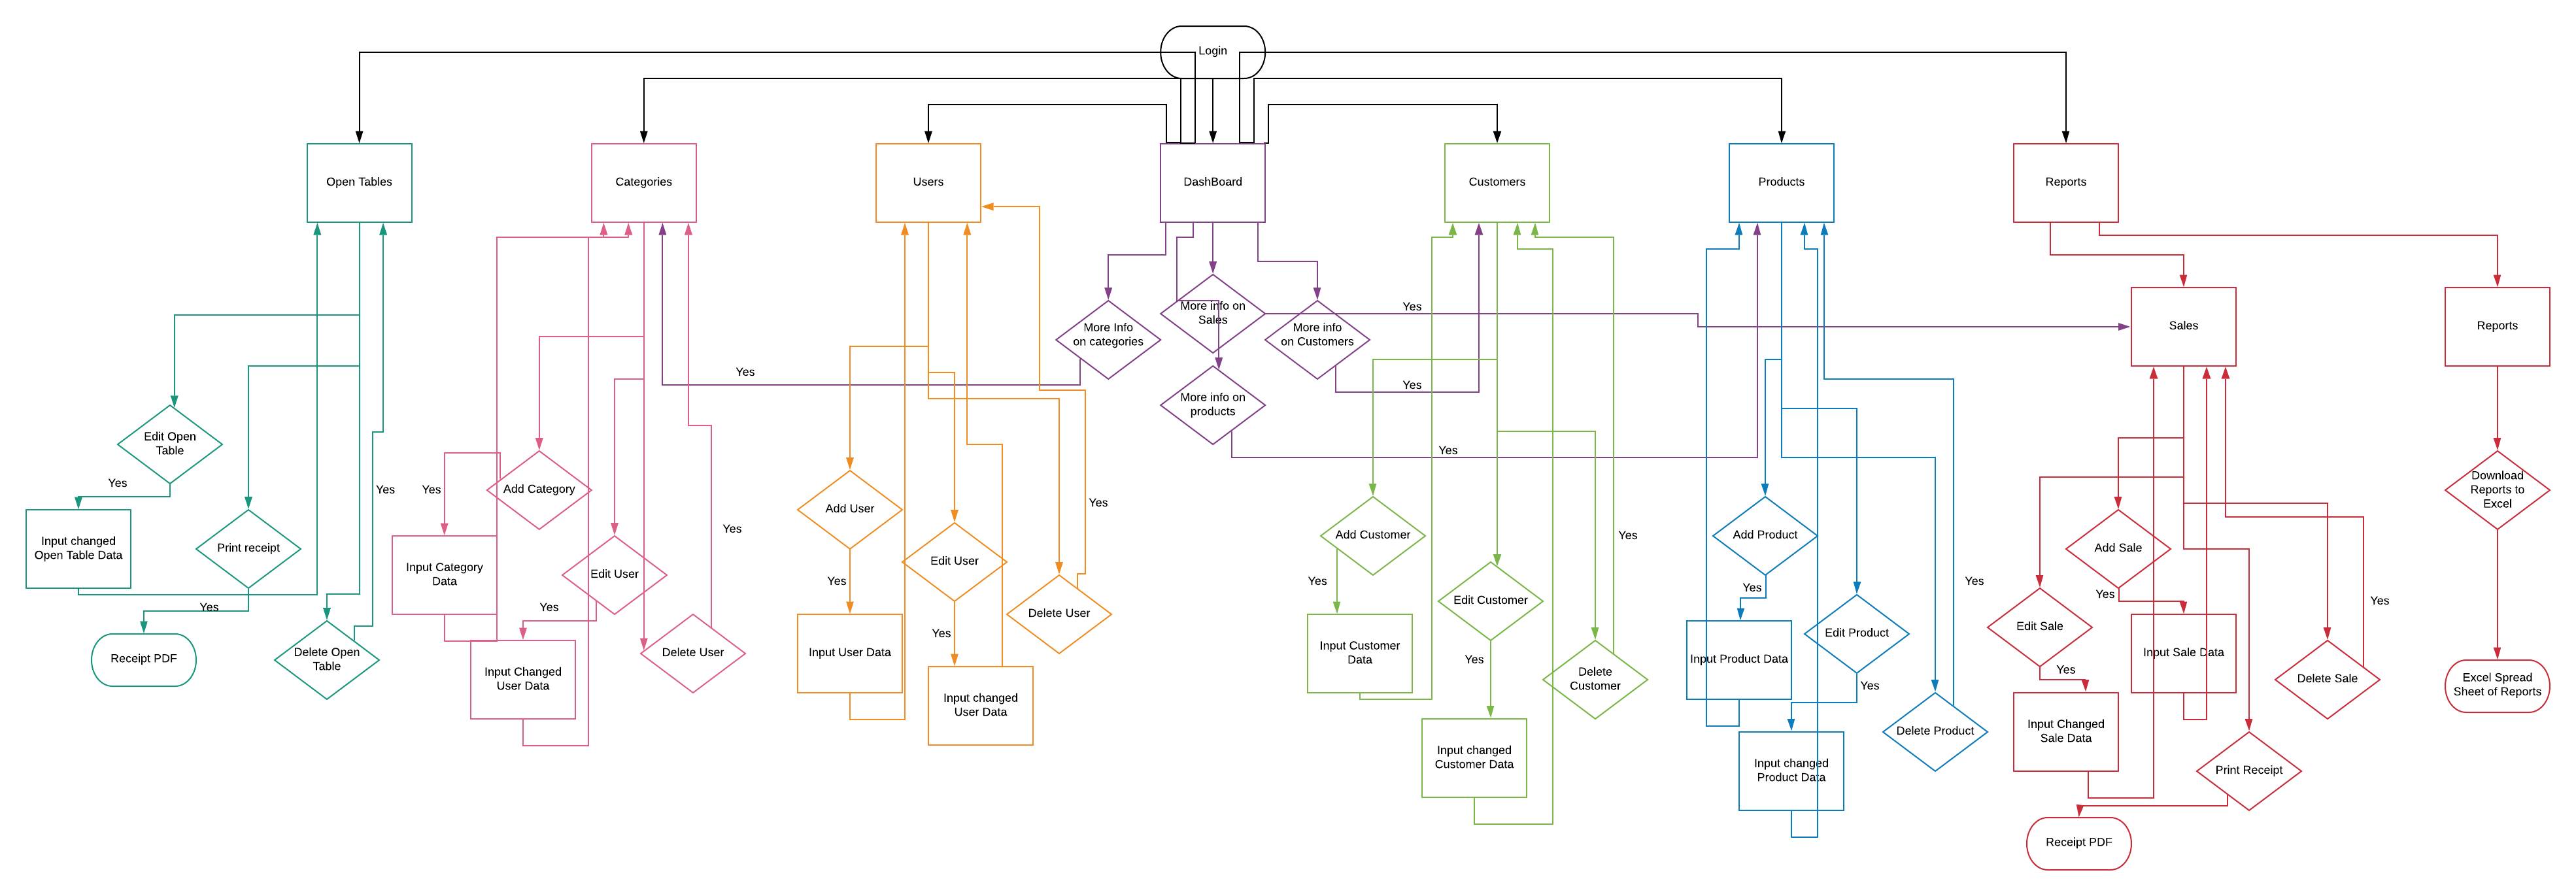
\includegraphics[width=0.9\textwidth]{Fig images/Flowchart.png}
\end{figure}

A flow chart is a diagram used to represent the process flow of an algorithm, problem, or some transaction within a business. Ideally, it is a diagram that depicts the process, system, and computer algorithm \cite{CHRT}. A flowchart is an essential tool for documenting the business system. It illustrates how we have managed to merge the POS and the RMS. It further enables developers in the future to improve or learn from the system. The flowchart has been designed to depict our system as it is indicating the different features as they are. 


\section{Ajax/Java Script}
In the creation of the Restaurant Management system Ajax played an essential role in the development as it was used in unison with JavaScript in fetching,editing and deleting data from the database tables.
\newline
\newline
Here is a walk through of some of the functions that are used and what is called when creating, editing and deleting categories that relate to Ajax/Java Script in our system.
\newline
\newline
We initially use PHP calls from the model and controller where it adds data to the database.
The controller asks for a response from he model as seen below to run the create category method which in turn adds a category.
\newline
\newline
Moving onto editing a category, when the edit category button is pressed the the categories.ajax.PHP file will fetch the category id for the specific category that is being edited from the database where the ID will then be used by the categories.js where once the fields are filled in the js file will send a POST to the database with the new edited information for the selected category.
\newline
\newline
Finally deleting a category starts off with pressing the delete category the categories.js file fetches the id of the desired category where once fetched the categories controller will take the category id and delete it in doing this the controller will once again send a request to the model to run the delete categories method, once successful the POS system will display a success message to the user.
 



\section{Chapter Summary}

This chapter covers system design in detail. Being a critical process in the entire build, the chapter details the same in the different sub-topics covering the entire planning, tools used consideration, and final structure. Diagrams have been used extensively in the chapter to illustrate the careful planning that ensured the project was a success. This includes a component diagram, entity-relationship diagram, till GUI, management GUI, and the flow charts. These diagrams further assist in the documentation of the project ensuring the entire build is represented and can be referred to for future research work or regular updates. 
\newline
\newline
The chapter further covers important features such as data storage. This has been covered extensively including, the type of database that will be used, its selection criteria, and characteristics. All these variables assist in ensuring the success of the project. Further, the chapter explains the business end of the system, illustrating how different design concepts assist in ensuring the project is successful. 
There are factors such as GUI and price display. The GUI has been stressed since it is the only section of the system that clients will interact with. The GUI has therefore been developed to ensure the customers have an easy time interacting with the system. The pricing concept allows the management to indicate the price of different products and services. This presents the client with a friendly portal where they can see the service or products that they opt for.
\newline
\newline
The chapter illustrates the importance of the management portal as well indicating how the complex back-end has been developed and simplified to a simple management GUI. This enables the business to be more streamlined by providing the management with clear statistical information about the enterprise. This chapter, therefore, illustrates the complex system design of the system and how it is integrated to ensure the business is successful. The next chapter, system evaluation documents in detail the expected performs of the system. The chapter will further extend the study and documentation of the system design indicating how the different selected tools and hardware contribute to the efficiency of the system. The chapter will evaluate the different design options take into consideration in this chapter illustrating their usability in a biased manner.

%References

%[1] 	M. Rouse, "Data Storage," Search Storage, May 2018. [Online]. Available: https://searchstorage.techtarget.com/definition/storage. 
%[2] 	codeacademy , "What is a Relational Database Management System?," Code Academy , 2020. [Online]. Available: https://www.codecademy.com/articles/what-is-rdbms-sql.
%[3] 	Oracle database, "Gartner Recognizes Oracle as a Magic Quadrant Leader in Database Management," Oracle Database, 2020. [Online]. Available: https://www.oracle.com/database/. 
%[4] 	Educba , "What is RDBMS?," Educba , 2020. [Online]. Available: https://www.educba.com/what-is-rdbms/. 
%[5] 	D. L. Soltesz, "The Advantages of a Relational Database Management System," TechWalla, 2020. [Online]. Available: https://www.techwalla.com/articles/the-advantages-of-a-relational-database-management-system. 
%[6] 	M. and Anas, "What is RDBMS and How it is better than DBMS?," Medium, 18 February 2018. [Online]. Available: https://medium.com/@anas18/what-is-rdbms-and-how-it-is-better-than-dbms-c25b211454d4. 
%[7] 	Lucidchart, "What is a Flowchart," Lucidchart, 2020. [Online]. Available: https://www.lucidchart.com/pages/what-is-a-flowchart-tutorial. 



